\documentclass[12pt,letterpaper]{article}
\usepackage[utf8]{inputenc}
\usepackage{tikz}
\usetikzlibrary{trees}
\usepackage[spanish, es-nodecimaldot]{babel}
\usepackage{amsmath}
\usepackage{color}
\usepackage{algorithm}
\usepackage[noend]{algpseudocode}
\renewcommand{\algorithmicrequire}{\textbf{Entrada:}}
\renewcommand{\algorithmicensure}{\textbf{Salida:}}
\usepackage{subcaption}
\usepackage{amsfonts}
\usepackage{hyperref}
 \hypersetup{
     colorlinks=true,
     linkcolor=blue,
     filecolor=blue,
     citecolor = blue,      
     urlcolor=cyan,
     }
\usepackage{amssymb}
\usepackage{listings}
\usepackage{color}

\definecolor{mygreen}{rgb}{0,0.6,0}
\definecolor{mygray}{rgb}{0.5,0.5,0.5}
\definecolor{mymauve}{rgb}{0.58,0,0.82}

\lstset{ 
  backgroundcolor=\color{white},   % choose the background color; you must add \usepackage{color} or \usepackage{xcolor}; should come as last argument
  basicstyle=\footnotesize,        % the size of the fonts that are used for the code
  breakatwhitespace=false,         % sets if automatic breaks should only happen at whitespace
  breaklines=true,                 % sets automatic line breaking
  captionpos=b,                    % sets the caption-position to bottom
  commentstyle=\color{mygreen},    % comment style
  deletekeywords={...},            % if you want to delete keywords from the given language
  escapeinside={\%*}{*)},          % if you want to add LaTeX within your code
  extendedchars=true,              % lets you use non-ASCII characters; for 8-bits encodings only, does not work with UTF-8
  firstnumber=1,                % start line enumeration with line 1000
  frame=single,	                   % adds a frame around the code
  keepspaces=true,                 % keeps spaces in text, useful for keeping indentation of code (possibly needs columns=flexible)
  keywordstyle=\color{blue},       % keyword style
  language=Octave,                 % the language of the code
  morekeywords={*,...},            % if you want to add more keywords to the set
  numbers=none,                    % where to put the line-numbers; possible values are (none, left, right)
  numbersep=5pt,                   % how far the line-numbers are from the code
  numberstyle=\tiny\color{mygray}, % the style that is used for the line-numbers
  rulecolor=\color{black},         % if not set, the frame-color may be changed on line-breaks within not-black text (e.g. comments (green here))
  showspaces=false,                % show spaces everywhere adding particular underscores; it overrides 'showstringspaces'
  showstringspaces=false,          % underline spaces within strings only
  showtabs=false,                  % show tabs within strings adding particular underscores
  stepnumber=2,                    % the step between two line-numbers. If it's 1, each line will be numbered
  stringstyle=\color{mymauve},     % string literal style
  tabsize=2,	                   % sets default tabsize to 2 spaces
  title=\lstname                   % show the filename of files included with \lstinputlisting; also try caption instead of title
}

\usepackage{amsthm}
\newtheorem{theorem}{Teorema}

\usepackage{graphicx}
\usepackage[inner=1.5 cm, outer = 1.5 cm, top=1 cm, bottom = 1.5 cm]{geometry}
\setlength{\parskip}{3mm}
\title{\textsc{Práctica 9: interacción entre partículas}}
\author{\textsc{Fabiola Vázquez}}
\renewcommand{\lstlistingname}{Código}
\setlength{\parindent}{0cm}

\begin{document}
\maketitle

\hrule
\section{Introducción}
En esta práctica \cite{elisapractica9} se tiene una cantidad \texttt{n} de partículas en un cuadro unitario, cada una de ellas posee una carga y una masa. El objetivo es verificar gráficamente que existe una relación entre los factores velocidad, carga y masa de las partículas. El experimento se lleva a cabo en el software R \cite{R} en un cuaderno de Jupyter \cite{jupyter}.

\section{Experimento}
Las partículas es posicionada normalmente al azar en el cuadro unitario y además estas poseen una carga que causa fuerzas de repulsión y atracción con las demás partículas si dos partículas tienen el mismo signo o diferente, respectivamente. Se desea añadir otro atributo a las partículas que afecte dicha interacción, este atributo es la masa y se considera el tamaño de esta en $\{0.2, 0.4, 0.6, 0.8, 1.0\}.$ 

En la figura \ref{im}
 \begin{figure}
 	\centering 
 	\begin{subfigure}[b]{0.3\linewidth}
 		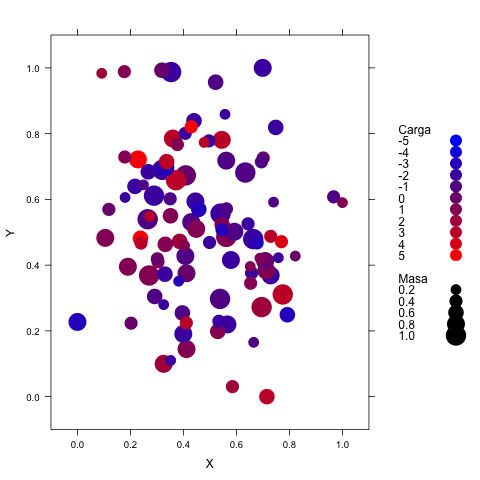
\includegraphics[width=\linewidth]{p9_t000.png} 		
 		\caption{Estado inicial.}
 		 		\label{1}
 	\end{subfigure}  \hfill
 	\begin{subfigure}[b]{0.3\linewidth}
 		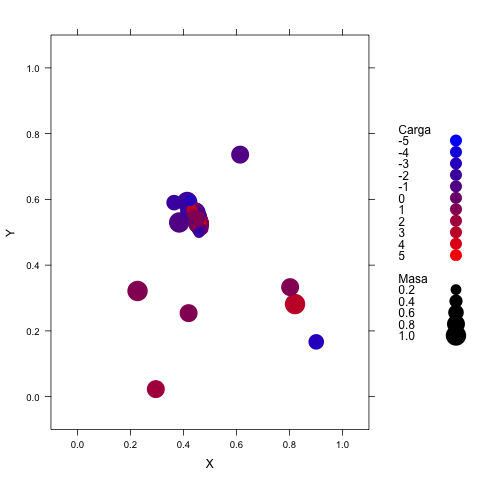
\includegraphics[width=\linewidth]{p9_t050.png} 		
 		\caption{Paso 50.}
 		\label{2}
 	\end{subfigure} \hfill
 	 	\begin{subfigure}[b]{0.3\linewidth}
 		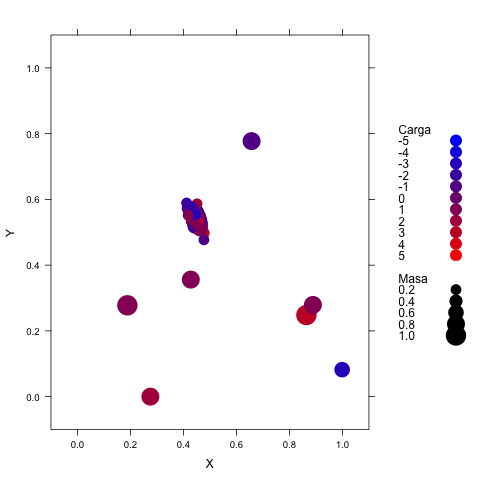
\includegraphics[width=\linewidth]{p9_t100.png} 		
 		\caption{Paso 100.}
 		\label{3}
 	\end{subfigure}
 	 	\caption{Interacción entre 100 partículas.} 
 	 		\label{im}
\end{figure} 

\begin{figure}
\centering
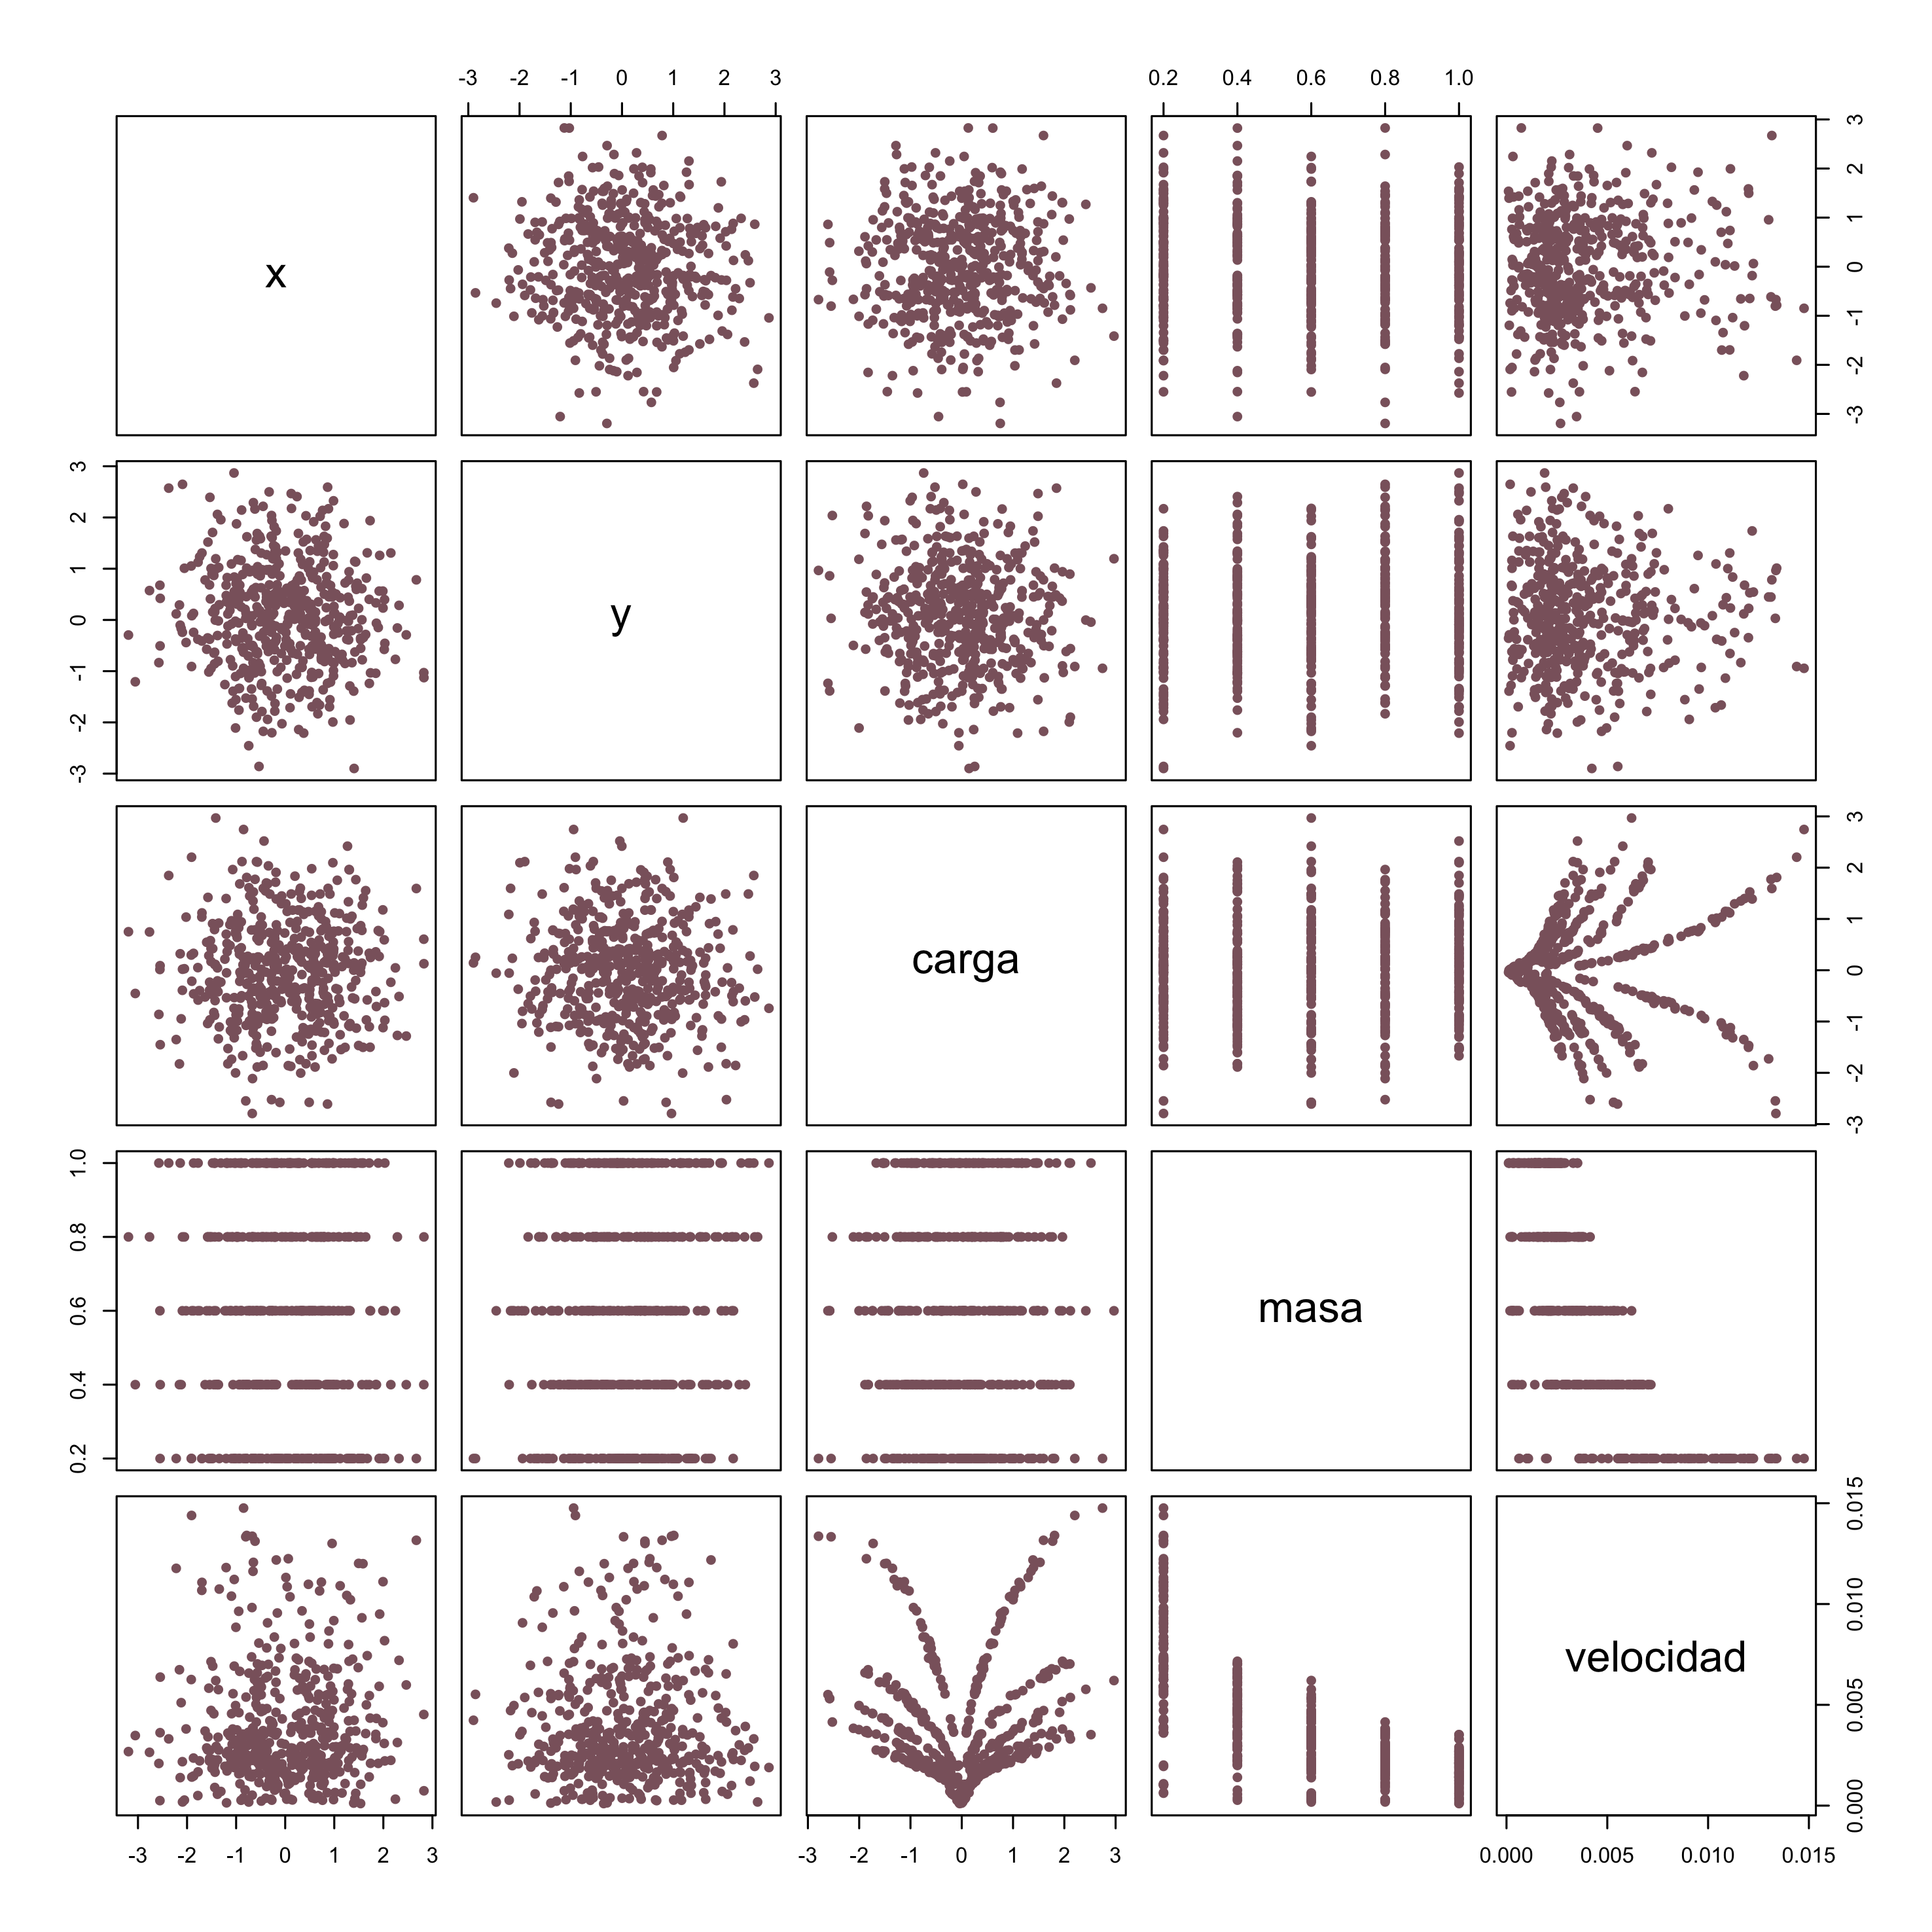
\includegraphics[width=\linewidth]{scatterplot.png} 		
 		\caption{Aplicación del filtro de Gauss a la imagen \ref{2}.}
 		\label{4}
\end{figure}
\bibliographystyle{plain} 
\bibliography{Referencias}


\end{document} 